\documentclass[nobib]{tufte-handout}

\title{Exercise session 9: Connectivity, planarity, colourings $\cdot$ 1MA020}

\author[Vilhelm Agdur]{Vilhelm Agdur\thanks{\href{mailto:vilhelm.agdur@math.uu.se}{\nolinkurl{vilhelm.agdur@math.uu.se}}}}

\date{6 November 2023}


%\geometry{showframe} % display margins for debugging page layout

\usepackage{graphicx} % allow embedded images
  \setkeys{Gin}{width=\linewidth,totalheight=\textheight,keepaspectratio}
  \graphicspath{{graphics/}} % set of paths to search for images
\usepackage{amsmath}  % extended mathematics
\usepackage{booktabs} % book-quality tables
\usepackage{units}    % non-stacked fractions and better unit spacing
\usepackage{multicol} % multiple column layout facilities
\usepackage{lipsum}   % filler text
\usepackage{fancyvrb} % extended verbatim environments
  \fvset{fontsize=\normalsize}% default font size for fancy-verbatim environments

\usepackage{color,soul} % Highlights for text

% Standardize command font styles and environments
\newcommand{\doccmd}[1]{\texttt{\textbackslash#1}}% command name -- adds backslash automatically
\newcommand{\docopt}[1]{\ensuremath{\langle}\textrm{\textit{#1}}\ensuremath{\rangle}}% optional command argument
\newcommand{\docarg}[1]{\textrm{\textit{#1}}}% (required) command argument
\newcommand{\docenv}[1]{\textsf{#1}}% environment name
\newcommand{\docpkg}[1]{\texttt{#1}}% package name
\newcommand{\doccls}[1]{\texttt{#1}}% document class name
\newcommand{\docclsopt}[1]{\texttt{#1}}% document class option name
\newenvironment{docspec}{\begin{quote}\noindent}{\end{quote}}% command specification environment

\include{mathcommands.extratex}

\begin{document}

\maketitle% this prints the handout title, author, and date

\begin{abstract}
\noindent
We consider the notion of $k$-connectivity, which is a more robust version of the normal notion of connectedness. Then, we investigate how one may draw a graph on paper, and learn about planarity. Finally, we think about colourings of graphs, both the vertices and the edges.
\end{abstract}

\section{Connectivity}

Imagine you are tasked with designing the Swedish electricity network. One of your interns comes to you with a terrible proposal which isn't even connected. You yell at them a bit, and they add a single edge to make it connected.

You yell at them again, telling them it needs to be \emph{more} connected than that. What if a Russian operative or an explosive moose destroys that single edge? Exasperated, your intern asks you what you mean by ``more connected'' than just being connected.

\begin{xca}
  What \emph{do} you mean?\sidenote[][-1cm]{There are many possible things you could mean by this, and there are many many papers about different versions. Try to think about what you are trying to defend against. 
  
  Are you worried about trees falling in storms and severing the electricity mains, or are you worried about Russians sneaking in and attempting to sabotage our infrastructure? Do these threats give you different notions of connectivity to strive for?}
\end{xca}

After much debating on this issue, considering storms and explosive meese and Russians, you get a call from Regeringskansliet. This is 2023: Russia is the only relevant threat, worrying about storms and climate change is for the future. You have intel that the Russian approach will be to blow up substations, not the wires themselves,\sidenote[][]{That is, they're destroying vertices, not edges.} and your goal is to maximize the number of substations they have to blow up in order to disconnect the entire network.

After some work, your team has come up with three candidate definitions of the \emph{connectivity} $\kappa(G)$ of a graph:
\begin{enumerate}
  \item A graph $G$ is $k$-connected if it has more than $k$ vertices, and for any set of less than $k$ vertices, removing those vertices does not disconnect $G$. The \emph{connectivity} $\kappa(G)$ is the greatest $k$ for which $G$ is $k$-connected.
  \item For any two vertices $v, w \in G$, we say that a set $X$ \emph{separates} $v$ from $w$ if $v, w \not\in X$ and every path from $v$ to $w$ contains at least one vertex from $X$. Let the minimum size of a set that separates $v$ from $w$ be denoted $\kappa(v,w)$, and then define the \emph{connectivity} of $G$ to be
  $$\kappa(G) = \min_{\substack{v, w \in V\\v\sim w \not\in E}} \kappa(v,w).$$
  \item For any two vertices $v, w \in G$, define $\kappa(v,w)$ to be the maximum size of a set of disjoint paths from $v$ to $w$.\sidenote[][]{That is, a set $W$ of paths from $v$ to $w$, such that for any two paths $P, P' \in W$, $V(P) \cap V(P') = \{v,w\}$.} Define the \emph{connectivity} of $G$ to be
  $$\kappa(G) = \min_{\substack{v, w \in V\\v\sim w \not\in E}} \kappa(v,w).$$
\end{enumerate}

\begin{xca}
  Prove that these definitions are in fact all equivalent.\sidenote[][]{The trickiest part of this is to show that the two different definitions of $\kappa(v,w)$ are equivalent. There is a clever quick proof of this using another flow graph construction (and perhaps a clever construction using duality for linear programming, of which max-flow min-cut is a special case), but it can also be done with a more hands-on approach. Make an attempt at it, but if you get stuck completely, move on to the other exercises.}
\end{xca}

After doing all this work, you get another call from Regeringskansliet. It turns out that the Russians have spent all their military resources on their invasion of Ukraine, so there's only one special ops team left to assault the Swedish electricity network. Thus, you only need to make sure the network is $2$-connected in order to thwart Putin.

\begin{xca}
  What can you say about the structure of a $2$-connected graph?\sidenote[][]{This exercise is intentionally very vague. We will be proving some structure theorems about $2$- and $3$-connected graphs in the next lecture, so this exercise is intended for you to get a feel for what they look like. Work on it until you run out of ideas, and then move on. Or look in last year's lecture notes for the theorem statements and try to prove them for yourselves, without looking at the proofs from last year.}
\end{xca}

\section{Planarity}

Consider the map of England and Wales given in Figure \ref{fig:england_wales_map}.

\begin{figure}
  \centering
  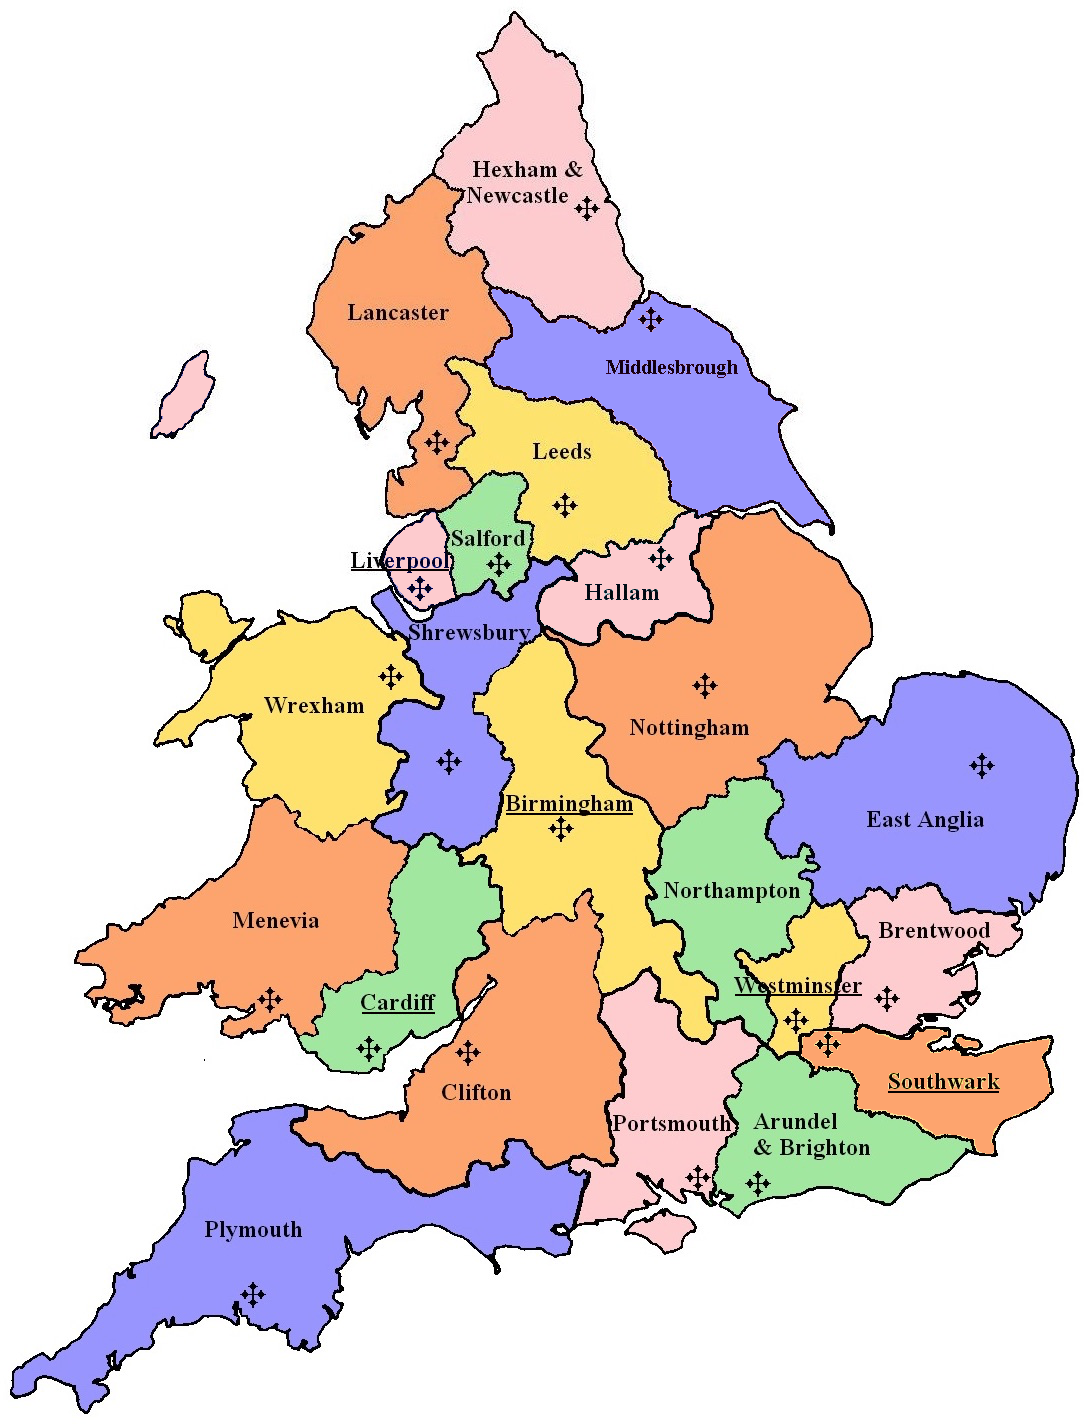
\includegraphics[width=0.8\textwidth]{graphics/L9_connectivity_planarity_colouring/england_wales_map.png}
  \caption[][1.5cm]{A map of England, divided into various areas of land. For the purposes of this exercise, ignore the existence of Anglesey, Isle of Man, Isle of Wight, and all other smaller islands, and pretend like the four-way meeting of Northampton, Westminster, Arundel \& Brighton, and Portsmouth doesn't exist -- let us say that Northampton and Arundel \& Brighton have a stretch of border, instead.}
  \label{fig:england_wales_map}
\end{figure}

There are two ways to turn this map into a graph. One way is to consider the vertices to be wherever three areas meet (considering the ocean/Scotland to be one area), and the edges to be the border lines between the areas. The other way is to consider the vertices to be the little cross icons (including an imaginary one in the ocean, or in Scotland), and draw an edge between two of them if their areas share a border.

\begin{xca}
  Draw both of these graphs.\sidenote[][]{Or, if you quite reasonably don't want to do this much drawing, pretend like a terrible flood has drowned all of the South, Midlands, and Wales, and just draw the two graphs for the northern parts of the map.}
\end{xca}

\begin{xca}
  We could of course have done this for any map. The crucial property of the graph we got by taking borders as edges is that no edges ever cross in our drawing of the graph. An embedding of a graph with this property is called \emph{planar}, and a graph which can be embedded in such a way is also called planar. A graph with a particular embedding fixed is called a \emph{plane} graph.

  Given any planar embedding of a graph, we can in fact derive another graph like the one we got by having the crosses be vertices and drawing edges between adjacent regions. Can you give a mathematical definition of this \emph{planar dual} of an embedding of a planar graph?\sidenote[][]{Consider in particular the fact that a planar embedding of a graph can have things happen that cannot happen if we got it from a map. In particular, what happens if the graph we are embedding has vertices of degree one or two? The map will, as you can convince yourself, always have minimum degree three.
  
  Another thing that can happen in general, but does not in the example we gave, is the situation at the France-Spain-Andorra borders.}
\end{xca}

\begin{xca}
  What happens if you repeat the process of taking the planar dual, taking the dual of the dual?
\end{xca}

\begin{xca}
  Given a planar graph, there can be more than one way of embedding it in the plane to get a plane graph. Do these different ways always give rise to the same planar dual?
\end{xca}

Finally, notice how we can in fact consider the plane graph $G$ and its planar dual $G^*$ to have the \emph{same} edge set, by identifying an edge in $G$ with the edge in $G^*$ which crosses it. So the following statement actually makes sense:

\begin{lemma}
  Suppose $G = (V,E)$ is some plane graph, and $G^* = (F, E)$ its planar dual. For any set of edges $S$, $(V, S)$ is a spanning tree if and only if $(F, E \setminus S)$ is a spanning tree of $G^*$.
\end{lemma}

\begin{xca}
  Prove this.\sidenote[][]{If you're feeling ambitious, you could also show that, if we attach weights to the edges, the minimum spanning tree of $G$ corresponds to a maximum spanning tree of $G^*$. If you're feeling less ambitious, skip this exercise -- we will give a proof in the lecture on this stuff.}
\end{xca}
%\bibliography{references}
%\bibliographystyle{plainnat}

\end{document}
